%%
%% Author: Jordan Osborn
%% 01/01/2019
%%

% Preamble
\documentclass[11pt]{article}

% Packages
\usepackage{amsmath, mathrsfs}
\usepackage{titling}
\usepackage{hyperref}
\usepackage[sorting=none, backend=bibtex]{biblatex}
\usepackage{graphicx}
\usepackage{float}
\usepackage{enumitem}

\let\oldhref\href
\renewcommand{\href}[2]{\oldhref{#1}{\bfseries#2}}


\addbibresource{report.bib}

\title{A new video analysis algorithm for the study of crowd dynamics}
\author{Jordan Osborn (jo357) Supervisor: Professor Pietro Cicuta (pc245)}
% Document
\begin{document}
\begin{titlingpage}
    \maketitle
\end{titlingpage}


\clearpage
\title{A new video analysis algorithm for the study of crowd dynamics}
\author{Supervisor: Professor Pietro Cicuta (pc245)}
\maketitle
\section*{Abstract}
%500 words overview
This project focuses on a new application of a technique called differential dynamic microscopy. DDM first appeared in 2008 \cite{ddm0} and has primarily found usage in the analysis of motion on a microscopic scale \cite{ddm1}. This project will make use of DDM to analyse macroscopic motion, specifically that of crowds. DDM has two primary forms, single-scale and multi-scale. Both will find usage in this project, single-scale DDM is used to analyse overall spatio-temporal dynamics, where-as multi-scale DDM can pick up temporal and spatial scales of synchronisation separately \cite{ddm1}. Multi-scale DDM achieves this separation by running single-scale DDM on multiple sub-sections of the footage at a range of "box sizes". A detailed description of the theory behind DDM is included in section \ref{section:theory}. DDM makes heavy use of Fourier transforms of the intensity differences between lagging frames. By transforming the intensity differences into the frequency domain, we can determine how the intensity decays as a function of the time lag between frames for each Fourier mode.  This data is then fitted to an intermediate scattering function (ISF) (analytical forms are known for specific types of motion), the functional form of the ISF determines what dynamical variables can be extracted from the data. This method has a significant level of computational complexity. Particular care was therefore taken in order to produce a satisfactory level of performance. The algorithm was implemented in the Rust programming language \cite{rust}, making heavy use of the GPU array parallelisation library Arrayfire \cite{arrayfire}. Data analysis was carried out using the standard Python data science stack (Python, numpy, pandas, matplotlib, scipy and sklearn). The algorithm was tested on simulated videos of Brownian motion before it was run on crowd motion videos in order to test its accuracy (more information can be found in section \ref{section:brownian}. Brownian motion was used as a test case as there is a known analytical form for the ISF (equation \ref{eqn:BrownianISF}). The expected functional form holds remarkably well (again see section \ref{section:brownian}) and so the algorithm was most likely correctly implemented. Analysis was carried out on two particular crowds types, Brownian-like (stationary motion e.g. stadium crowd where motion is constrained to oscillation about seat location) and Swimmer-like (directional crowd motion e.g. marathon running) (see section \ref{section:crowdtypes} for further details). The crowd videos were assigned one of these two categories or left uncategorised. Data was collected for every video but data analysis was only carried out on the Brownian-like and Swimmer-like crowds. This was done as there is at least an approximately known form of the ISF for Brownian/Swimmer like crowds (the microscopic Brownian \ref{eqn:BrownianISF} and Ballistic \ref{eqn:BallisticISF} ISFs) where as for the uncategorised crowds it was not clear what form of ISF should be selected. Other crowd types and the form of their ISFs could be an avenue for further research. The results and their discussion (single-scale and multi-scale DDM) for Brownian and Swimmer like crowds can be found in sections \ref{section:results} and \ref{section:discussion}. It is hoped that this report will demonstrate the suitability of DDM for the analysis of macroscopic motion (crowds). With further research (crowd types and their associated ISFs) and development (focusing on algorithmic optimisation and usability) DDM might find usage in real-time crowd safety monitoring systems at stadiums, in shopping malls, on crowded streets and more.

\clearpage
\tableofcontents
% TODO: 5000 Words 

\clearpage
\section{Introduction}
In this project the technique of Differential Dynamic Microscopy will be applied to videos of crowd motion. This technique provides information about the dynamical behaviour of objects in a video without the use of image segmentation. DDM was first carried out in 2008, to analyse the dynamics of colloidal particles in Brownian motion \cite{ddm0}. A video of colloidal particles will be analysed and will act as a test case for the code developed in this project. Differential Dynamic Microscopy has primarily been used to analyse the motion of microscopic particles \cite{ddm1} \cite{ddm2}. This project was undertaken in order to determine the applicability of DDM to macroscopic motion i.e. crowd motion videos. A literature review will be carried out in section 2, but this will mainly be centred around the microscopic applications of DDM as prior literature is not available for the application of DDM to macroscopic motion. The code developed as a part of this project is intended to act as a reference for further development (e.g. for real time commercial crowd analysis) and so has been developed with execution speed as well as accuracy as a priority. Certain design decision were undertaken to achieve this. Further discussion about implementation will be carried out in section 3.
\\\\
DDM is used to extract dynamical information from videos by analysing the Intensity profile (in k-space) of the differences between a starting frame and lagging frames. This intensity is a function of wave-vector q and $\tau$ the time delay between frames. By fitting this curve to the expected image structure function we can extract dynamical information about the system. A detailed discussion of the theory behind DDM will occur in section 3. (The information extractable from a DDM analysis is sensitive to the particular dynamics of the system for example for particles undergoing Brownian motion it is possible to extract the size of the diffusing particle \cite{ddm1}.)
\\\\
There are two primary types of DDM analysis. Single-scale DDM and multi-scale DDM. Single-scale DDM performs DDM analysis on the entire image and so picks up a combination of the spatial and temporal scales of synchronisation \cite{ddm2}. Where as Multi-scale DDM performs DDM analysis on individual tilings of the image from a full-scale image down to the smallest tile size (determines the mini-mum wave-vector that can be compared across tiles) \cite{ddm2}. In this way spatial and temporal scales of synchronisation can be picked up separately. A more in-depth description of the two methods will take place in sections 3 and 4.  
\\\\
Each type of analysis will yield different pieces of dynamical information. Both methods will be run on a large database of approximately 400 videos \cite{crowdMotionDB}. The data will then be analysed, dynamical information will be extracted and then compared to that extractable by eye (for select videos). This analysis and discussion will take place in sections 5 and 6.
\\\\
DDM has the potential to be used to implement real-time analysis of crowd motion without the use of image segmentation, or the use of machine learning (expensive datasets and long training periods). Section 7 contains an in depth discussion about the future of DDM as applied to the analysis of crowd motion. The hope is that DDM might one day be used to help implement real-time crowd safety/monitoring systems in environments such as public transportation, stadiums, city centres etc.

\clearpage
\section{Literature Review}
DDM is a relatively recent development originating in the paper "Differential dynamic microscopy: Probing wave-vector-dependent dynamics with a microscope" in 2008 \cite{ddm0}. In this paper the technique was used to attempt a characterisation of the dynamics of colloidal particles undergoing Brownian motion. DDM was first used to determine the diffusion coefficient of colloidal particles suspended in a liquid medium \cite{ddm0} \cite{ddm_maths}. This is likely due to the known form of the intermediate scattering function for Brownian motion equation \ref{eqn:BrownianISF}. If the viscosity of the liquid is known DDM can also be used to determine the size of the diffusing particles \cite{ddm1} and vice versa. 
\\\\
Due to DDMs insensitivity to static features of the sample, DDM has found a use in the analysis of hindered diffusion \cite{nanoposts}. Static nano-posts in a square periodic array were used to confine diffusing particles. Using DDM the diffusion coefficient as a function of confinement strength was determined.
\\\\
% ddm2 
Multi-scale DDM has been used to study the collective dynamics of cilia \cite{ddm2}. These cilia beat at a well defined frequency. Through the application of multi-scale DDM temporal and spatial coherence scales of cilia dynamics can be found \cite{ddm1}. In a system that has a spatial scale for collective motion (cilia) we would expect that scale to emerge as a feature when comparing the dynamics across tile sizes \cite{ddm1}. And so by seeing how the intensity profiles vary with respect to tile size it is possible to determine spatial coherence of the collective motion.
\\\\
%bacterial_motility
DDM has also been used to analyse bacterial motility \cite{bacterial_motility}. In this paper the motion of isotropic "swimmers" (e-coli) was analysed. DDM was used to extract the swimming speed distribution of the bacteria and also their diffusion properties. In this case the data from DDM is fitted to an intermediate scattering function of a similar form to equation \ref{eqn:BallisticISF}, however the fitted form is slightly more complicated in that it takes account of the possibility that only a fraction of "swimmers" are motile and also that the swimmers follow some specified speed distribution \cite{bacterial_motility}.
\\\\
% only applied to microscopic motion so far this is entirely new, ddm1 cite for a review of ddm.
An in-depth literature review of DDM was carried out in 2017 \cite{ddm1}. This review focused on the areas in which DDM has been applied, it found that so far DDM has only been used to analyse microscopic dynamics, specifically biological samples suspended in a liquid medium. Further research yielded no results for DDM being used to analyse macroscopic dynamics. This project therefore offers original research on the method of DDM with no evidence of prior literature on this application. The results from past experiments will be used as test cases (primarily Brownian motion) to verify the validity of the code written. Results from this project could provide the motivation to carry out research on further applications of DDM.

\clearpage
\section{Theory}
\label{section:theory}
DDM or Differential Dynamic Microscopy is a method that can be used to analyse an image sequence by taking a difference between two images (removes static features and retains only motion/differences between frames), and then taking the 2D spatial Fourier transform (using a 2D FFT algorithm \cite{fft}) of this difference to obtain an image structure function.
From this function many properties of the motion can be determined \cite{ddm1}.

\subsection{Mathematics}
Defining d the image structure function (in position space) as
\begin{equation}
    d(\textbf{r}, t_0, \tau) = I(\mathbf{r}, t_0 + \tau) - I(\mathbf{r}, t_0)
\end{equation}
Where the function $\textit{I}$ encodes the 2D projection of the scene along the optical axis of the camera (i.e the image intensity) as a function of position and of time.
This intensity could well be in colour (tuple of 3 intensities for red, green and blue) or could be in greyscale. Colour information may provide extra information about motion but may also be an artefact produced by lighting effects. Greyscale images would provide the necessary motion information and would not be vulnerable to the issues colour images may pose (more computational complexity, does a colour change really indicate motion etc.)

\begin{equation}
    \mathscr{F} (d(\textbf{r}, t_0, \tau) ) = \mathscr{F} (I(\mathbf{r}, t_0 + \tau) - I(\mathbf{r}, t_0)) = \mathscr{F}(I(\mathbf{r}, t_0 + \tau)) - \mathscr{F}(I(\mathbf{r}, t_0))
\end{equation}

The second equality results from the linearity of the Fourier transform and reduces computational complexity as it allows you to cache Fourier transforms at each time and then compute their difference.
This reduces the number of Fourier transforms you need to compute, hence provides a computational optimisation.\cite{ddm2}
We now have

\begin{equation}
    d(\textbf{q}, t_0, \tau) ) = \mathscr{F}(I(\mathbf{r}, t_0 + \tau)) - \mathscr{F}(I(\mathbf{r}, t_0))
\end{equation}

Where $\textbf{q}$ is the 2D wave vector $(q_x, q_y)$.
Simplifications can be made if you can make some assumptions about the properties of the image, including isotropy and that motion is indifferent about the reference time (can average for all $t_0$) \cite{ddm1}.
\\\\
The wave-vectors can be used to derive a wavelength $(\lambda = \frac{2\pi}{|\textbf{q}|})$ which gives you the length scale probed by a particular mode.
Information about the system's dynamics can be obtained by looking at how the amplitudes of the Fourier modes for each q changes with the time differences between frames $\tau$ \cite{ddm2}.
\\\\

It has been shown in general that the image structure function takes the form given below \cite{ddm1}.
\begin{equation}
	I(\textbf{q}, \tau) = A(\textbf{q}) \cdot (1 - f(\textbf{q}, \tau)) + B(\textbf{q})
\end{equation}

Where $f(\textbf{q}, \tau)$ is the normalised "intermediate scattering function" as commonly measured in dynamic light scattering experiments \cite{DLSPecora}. A few analytical forms for f are known including Brownian motion and Ballistic motion \cite{DLSPecora}. The function f "characterises how quickly structure is lost over length scales ~ 1/q"\cite{ddm1}. The parameters A(\textbf{q}) and B(\textbf{q}) are functions related to the static scattering properties of the sample, to the details of the imaging process optics and to the noise in the acquisition \cite{ddm1}. These are just going to be considered as fitting parameters but some useful information can be extracted from them \cite{ddm1}. All interesting dynamical properties are often completely captured by $f(\textbf{q}, \tau)$ \cite{ddm1}. The intermediate scattering function f is the spatial Fourier transform of the Van-Hove self space-time correlation function \cite{DLSPecora}.

\begin{equation}
	f(\textbf{q}, \tau) = \mathscr{F} (G(\textbf{r}, \tau)) = \int d^3 \textbf{r} e^{i \textbf{q} \cdot \textbf{r}} G(\textbf{r}, \tau)
\end{equation}

The Van-Hove equation is the probability distribution for a particle with position $\textbf{R}_j(t)$ to suffer a displacement $\textbf{r}$ in a time $\tau$ \cite{DLSPecora}.

\begin{equation}
	G(\textbf{r}, \tau) = \left\langle \delta (\textbf{r} - [\textbf{R}_j(t) - \textbf{R}_j(0)]) \right\rangle
\end{equation}

It is easy to see through the definitions above how dynamical information about the system can be extracted from the form of the intermediate scattering function.
\\\\
Now this is a complicated equation and so has only been solved analytically for a few cases. One of which is Brownian motion. In the case of Brownian motion the ISF has been shown to be

\begin{equation}
\label{eqn:BrownianISF}
	f(\textbf{q}, \tau) = e^{- \tau / \tau_c(\textbf{q})} = e^{- \tau / (\frac{1}{D_T |\textbf{q}|^2})}
\end{equation}
where $D_T$ is the translational diffusion coefficient \cite{ddm1}. If we then fit this to data from videos behaving in a similar manner to Brownian motion we should then have $\tau_c$ as a function of $|\textbf{q}|$. Plotting this data on a log-log plot we should then see the characteristic form predicted by the equation above
\begin{equation}
\log{\tau_c} = -2 \cdot \log{|\textbf{q}|} - \log{D_T}
\end{equation}
By comparing the measured gradient to -2 we can see how valid the assumption of Brownian motion is. And from the y-intercept we can also derive a prediction for the translational diffusion coefficient $D_T$.
\\\\
Another solved case is that of Ballistic motion. This form is derived on the assumption of an isotropic collection of motile "swimmers" that also undergo Brownian motion as they travel. The form of the intermediate structure function in this case is 

\begin{equation}
\label{eqn:BallisticISF}
	f(\textbf{q}, \tau) = sinc(|\textbf{q}| \cdot v \cdot \tau) \cdot e^{- \tau / \tau_c(\textbf{q})}
\end{equation} \cite{DLSPecora}.

Systems that show similar behaviour to ballistic motion should have a similar ISF, from the ISF we should therefore be able to extract the velocity of the crowd from the first peak in the intensity profile.
\\\\
A related method called multi-scale DDM (this project will make heavy use of this method) picks up temporal and spatial scales of synchronisation separately (normal single-scale DDM only picks up a combination).
In multi-scale DDM you perform a single-scale DDM over a whole series of different tilings of the image \cite{ddm1}. These tilings are chosen so that windows vary from a full scale image down to the smallest tile size (determines the minimum wave-vector that can be compared across tiles) (usually log spaced) \cite{ddm1}.
To reduce the number of tiles that need to be computed you can select only the tiles showing the most activity, an equation that can determine if a tile exceeds a threshold activity is
\begin{equation}
    \Sigma_{\textbf{r} \in tile} \sigma(\textbf{r}) = \Sigma_{\textbf{r} \in tile} \sqrt{\frac{\Sigma_{[t_0, t_0 + \tau]} (I(\mathbf{r}, t) - <I(\mathbf{r}, t)>)^2}{N - 1}} > \sigma_{threshold}
\end{equation}

Which sums all of the standard deviations (computed over the time period $\tau$) of the intensities at each position in the tile and then checks if this sum is greater than some threshold standard deviation.
If it is a valid inequality then that tile is said to be "active" otherwise it is "inactive".\cite{ddm2}
This is a very rudimentary activity classifying function.
There are other ways that a tile's activity can be classified which may need to be investigated.
\\\\
In the cross comparisons between the tiles of different sizes the scale of the collective motion should emerge \cite{ddm1}.
Other properties of the motion should emerge by studying how tau varies as a function of the wave-vector amplitude \cite{ddm1}.
\\\\
DDM can be carried out as a fully automated process, as long as the expected form of the system's dynamics is known beforehand. This means that once a family of dynamics is chosen, the DDM data can be fitted to the expected functional form and dynamical information can be extracted, all without the input of a user  \cite{ddm1}.

\subsection{DDM Example - Brownian Motion}

\begin{figure}[H]
\centering
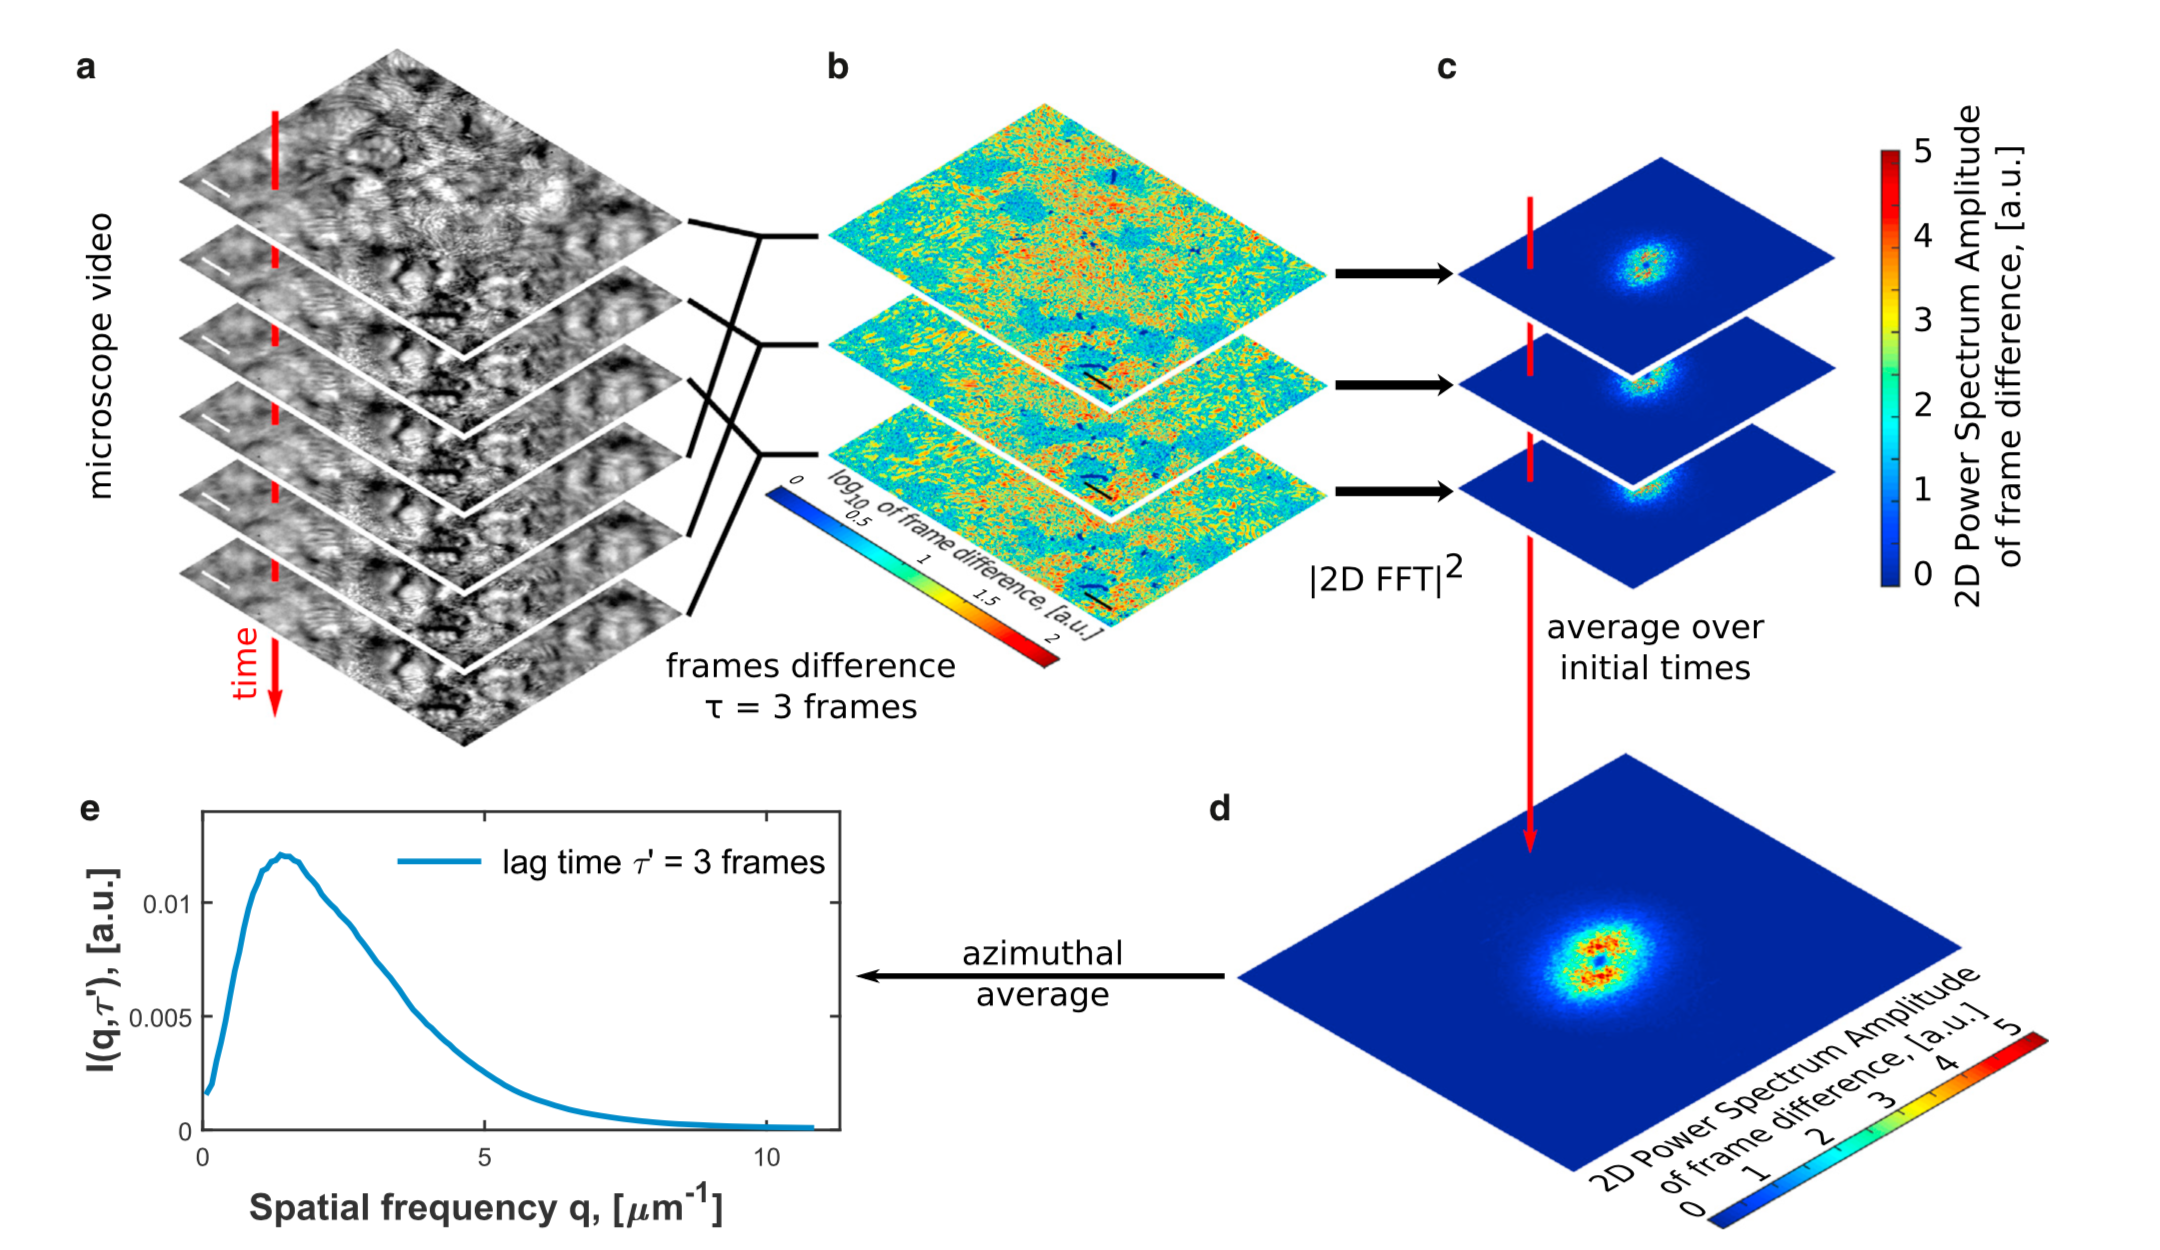
\includegraphics[height=4.5cm]{images/ddmpic.png}
\caption{Provides an overview of the DDM method as applied to the analysis of collective dynamics in ciliated cells.\cite{ddm2}}
\end{figure}

\begin{enumerate}[label=\alph*]
\item we take a video of the motion we wish to analyse and convert each frame into a 2D array of gray-scale pixel intensities.
\item for each starting frame in the video we take the difference between the pixel intensities of that frame and all lagging frames. $ \tau $ 
denotes the temporal separation of the two frames ( $ \tau = 3 $ frames,  is shown for various start times $ t_0 $). We denote each of these differences $ d(\underline{x}, t_0, \tau) $.
\item the 2D spatial Fourier transform of $ d(\underline{x}, t_0, \tau) $ is then taken for all combinations of $ t_0 $ and $ \tau $. Giving us d as a function of wave-vector instead of position. $ d(\underline{q}, t_0, \tau) $. We then take the the modulus squared of each Fourier transform giving us a power spectrum $I(\underline{q}, t_0, \tau) = |d(\underline{q}, t_0, \tau)|^2$.
\item because the system is stationary (power spectrum should be independent of $t_0$ and should only depend on $\tau$) we therefore take the average of the Fourier transforms over each $t_0$. This allows us to remove the dependence of $t_0$ from I and also reduce the effects of experimental uncertainty.
\item in the current case the system is also isotropic and so we can then take the azimuthal average of the 2D power spectrum. This means the power spectrum is now only a function of the modulus of the wave-vector q. $I(q, \tau)$
\item the expected functional form (for Brownian Motion) of this power spectrum has been proven to be $I(q, \tau) = A(q) \cdot (1 - e^{-\tau / \tau_c (q)}) + B(q)$ \cite{DLSPecora}. The physically interesting information is contained within $\tau_c$. $\tau_c$ for Brownian motion has been shown to equal $(D \cdot q^2)^{-1}$. Fitting the data (at each $\tau$) to this functional form and then extracting the value of $\tau_c$ as a function of q will yield the diffusion coefficient D. Plotting $log(\tau_c)$ against $log(q)$ should show a relationship of the form $y = -2\cdot x - log(D)$. The diffusion coefficient can then be used to find other pieces of information about the system including the size of the colloidal particles as there is a known relationship $D=\frac{k_B T}{6 \pi \eta R}$ between these two variables \cite{wynot_2002}.
\end{enumerate}

\subsection{Types of Crowd}
\label{section:crowdtypes}
In this project we will be focusing primarily on two types of crowd. Crowds which are "stationary" for example people sat inside a stadium. Motion is restricted to oscillations around the person's average location. We term this crowd type "Brownian-like". The other type is that where the crowd shows some overall direction of travel. For example runner's in a marathon. We term this type of crowd "Swimmer-like". Videos have been typecast in to one of these two categories or neither (if they show a different type of motion). We expect the ISF for videos of a particular category to be similar (albeit with different values for the fit parameters) i.e of the same functional form. For the Brownian-like crowds we will try a fit of the type expected for Brownian motion (equation \ref{eqn:BrownianISF}). And for Swimmer-like crowds we will try a fit of the expected type for ballistic motion (equation \ref{eqn:BallisticISF}).

\clearpage
\section{Implementation}

DDM is a very computationally intensive algorithm, in order to approach real-time speeds it was necessary to focus on producing an optimal implementation from the start. Certain design decisions were primarily made in order to facilitate the required optimisations. The design decisions and how they were made will be explained in the following paragraph. An outline of the algorithm pipeline will then complete this section.
\\\\
\subsection{Tools and Technologies}
Because of the nature of the DDM algorithm (mainly large array manipulations) it was decided that the code should target GPUs due to their suitability for highly parallelised array based Mathematics. An Nvidia Jetson TX2 was provided as a development board (will now be referred to as just the Jetson). The Jetson is a powerful, energy efficient development board with an embedded GPU\cite{jetson}. The Jetson GPU can be coded with the programming language CUDA, but after carrying out initial research \cite{cuda_book} it was decided that writing raw CUDA code by hand would be a significant undertaking and so other avenues to utilise GPU parallelism were explored. After careful consideration the library ArrayFire was selected as it offered optimised algorithms for several backends (GPU: CUDA/OPENCL and CPU: All)\cite{arrayfire}. This was an important feature as it meant it would be possible to avoid timely reimplementations of various algorithms and also that rapid prototyping on any development machine was possible due to the available CPU and OPENCL backends.
\\\\
Due to the selection of Arrayfire (availability of language bindings), the focus on speed and my own programming knowledge the selection of programming language was effectively limited to C++ or Rust \cite{rust} (for core algorithm implementation). Rust is a relatively recently developed programming language with a focus on speed, safety and concurrency. I selected Rust for the core of the algorithm implementation as it allows you to develop concurrent code in a much easier and safer way than C++, this is important so that the algorithm will not be bound by the CPU (passing data around, reading frames, sequential operations). Due to the relative immaturity of Rust language bindings for popular libraries are still in their infancy. This required me to create a small C++ library to expose language bindings for OpenCV over a C ffi (foreign function interface). OpenCV is used to capture video streams from files, cameras, urls etc. Frames from these streams are then sent into the DDM algorithm as they become available. This level of optimisation allows the bulk of the algorithm to run in less time than the length of the video (even using the CPU backend). There however is a significant slowdown associated with the radial averaging of the Fourier Transforms during the DDM algorithm. This slowdown prevents the algorithm from running in real-time but with further development it is anticipated that radial averaging can be optimised as the algorithm used currently only uses very rudimentary techniques (time limitations have so far prevented the implementations of these optimisations). After completion of the DDM algorithms the raw data is added to an SQlite database to allow efficient querying of the available data.
\\\\
Again due to time limitations and the immaturity of the Rust library ecosystem all data analysis (image structure function fitting etc. The ISFs are often not linearisable which means we have to resort to non-linear least-squares regression, scipy provides built in methods for this based on the Levenberg-Marquardt algorithm \cite{scipy_fit}.) and data exploration was undertaken using Python (numpy, scipy, matplotlib, pandas, sqlite, etc.) and Jupyter Notebooks. If time permitted a custom curve fitting solution would have been added to the Rust codebase so that the algorithm could run as a totally self contained executable. This custom fitting solution would need to be implemented if DDM were to find an application in real-time autonomous crowd monitoring systems.
\\\\
Software development best practices were followed throughout development. The project was version controlled using Git, continuously integrated using \href{https://travis-ci.com}{TravisCI} and a custom docker image, the set-up of both a mac OS and Linux based development environment was documented in detail, and core algorithms were benchmarked and tested in depth.
\\\\
\subsection{Algorithm Pipeline}
\begin{figure}[H]
%algorithm pipeline	
\centering
\noindent \includegraphics[height=0.7\paperwidth, width=0.6\paperwidth]{images/algo-pipeline.png}
\caption{Flow chart of the algorithm structure used in this project.}
\end{figure}
 
\clearpage
\section{Results}
\label{section:results}
%TODO: All multi-ddm and analyse
\subsection{Brownian Motion}

\subsection{Single-Scale DDM}
\subsubsection{Stationary Crowds - Brownian Like}

\subsubsection{Directional Motion - Swimmer Like}

\subsection{Multi-Scale DDM}
\subsubsection{Stationary Crowds - Brownian Like}

\subsubsection{Directional Motion - Swimmer Like}

\subsection{Performance}

\clearpage
\section{Discussion}
\label{section:discussion}
\subsection{Brownian Motion}
\label{section:brownian}

\subsection{Single-Scale DDM}
\subsubsection{Stationary Crowds - Brownian Like}

\subsubsection{Directional Motion - Swimmer Like}

\subsection{Multi-Scale DDM}
\subsubsection{Stationary Crowds - Brownian Like}

\subsubsection{Directional Motion - Swimmer Like}

\subsection{Performance}
\label{section:performance}
%graphs and data

\clearpage
\section{Future}
\subsection{Comparisons}
There are many methods that can be used to analyse motion within videos. Some examples are outlined and compared with DDM in the sections below.
\subsubsection{Image Segmentation}
In image segmentation an image is partition in to a set of segments. The image is split in to segments that have certain characteristics (colour, intensity, etc.) and could be chosen algorithmically or manually. This is carried out in order to simplify the image and hence reduce the complexity of any subsequent analysis. \cite{computer_vision_book} An example of image segmentation would be object detection using the gradient of intensity to detect object boundaries (edges) using a Sobel filter \cite{sobel}. Image segmentation can be carried out using a variety of algorithms including k-means clustering (an unsupervised technique) \cite{segmentation_kmeans}. K-means clustering is carried out by picking k centres (categories) then putting each segment in the category that minimises the difference between the cluster center and the segment. The cluster centres are then re-computed by averaging over all points in the cluster and the previous step is repeated until convergence. Segmentation could be carried out on moving objects by carrying out these techniques on the difference between successive frames (static background should be removed).
\\\\
Most image segmentation algorithms are very computationally intensive and some even require manual input. DDM however offers solutions to both of these problems. DDM can offer dramatic speed improvements due to its highly parallel nature and can even be made to run fully autonomously (once an ISF is selected). DDM focuses on more fundamental properties of the motion and is backgrounded in physics (fitting to a derived ISF) whereas with many image segmentation techniques the focus is on a straight analysis of the image intensity field and can be incredibly sensitive to the properties of the video (leading to over-under segmentation etc.) \cite{computer_vision_book}. 

\subsubsection{Neural Networks}
Neural networks offer some unique benefits over DDM in that they can be trained to find specific objects in an image and so can be used to directly count the number and location of different objects \cite{yolov3}. The main drawback is that these predictions will only be as good as the quality of your dataset. High quality data is often not available and when it is it is usually very expensive to procure. The larger your training dataset the longer it will take to train (usually with the benefit of more accurate predictions). Often training algorithms will require a form of supervised learning, for example the images will need to be tagged with the objects they contain. This is a time consuming process. However once the model is trained it can usually produce predictions in a reasonable time frame. However if detection of a new type of object is required the model will need to be retrained, often with a new dataset. \cite{tensorflow} DDM requires no such training data and can therefore be used with zero training time on any type of motion (once an ISF is selected). These two methods are however not at odds with one another, DDM can't be used to track objects as it doesn't really have a notion of the individual constituents of the system. It is primarily focussed on extracting dynamical information of the entire system or average information about the individual constituents. Neural networks however can be used to locate and track individual objects between frames. It however is not really applicable to the extraction of dynamical information. These two methods could therefore be used in tandem to track and analyse the motion inside crowds.

\subsubsection{Particle Image Velocimetry}
Is a technique that is more appropriate for comparison with microscopic applications of DDM. However it does offer some insight in to the benefits of DDM analysis. PIV is used to obtain velocity and related information about the flow of fluids. It achieves this through the introduction of tracer particles. These particles are assumed to follow the overall flow of the fluid. The fluid is illuminated and the tracer particles are tracked to measure the velocity field of the flow \cite{piv}. This method therefore requires pre-preparation of the system that is to be studied, DDM however can be applied to pre-recorded motion and does not require any special conditions to be set-up before it can be used. 

\subsubsection{Optical Flow}
"Optical flow is the distribution of apparent velocities of movement of brightness patterns in an image" \cite{optical_flow}. It can arise due to relative motion between an observer and the objects in a scene. Optical flow can give information about the spatial positioning of objects and the rate of change of the arrangements of these objects. "Discontinuities in the optical flow can help in segmenting images into regions that correspond to different objects" \cite{optical_flow}. However objects may be moving but exhibit no change in brightness, this method will therefore not be sensitive to this sort of motion. It is possible to determine the velocities of the motion from the brightness gradients computed from the footage.
\\\\
The equation that is used to determine these velocities is derived under the assumption that the pixel intensity of a moving object ($x \rightarrow x + dx, y \rightarrow y + dy, t \rightarrow t + dt $) is unchanged and that neighbouring pixels have similar motion \cite{optical_flow_opencv}.
\begin{equation}
I(x, y, t) = I(x + dx, y + dy, t + dt)
\end{equation}
Taking the Taylor expansion of this equation and only retaining terms up to first order.
\begin{equation}
I(x, y, t) = I(x, y, t) + \frac{\partial I}{\partial x} dx + \frac{\partial I}{\partial y} dy + \frac{\partial I}{\partial t} dt
\end{equation}
After rearranging and then taking the time derivative we arrive at the desired equation.
\begin{equation}
0 = \nabla I \cdot \textbf{v} + \frac{\partial I}{\partial t}
\end{equation}
 
There are some notable caveats of this method which are outlined in detail in \cite{optical_flow}. The method requires you to solve a partial differential equation thus necessitating implementation of some constraints in order to fully determine the motion. It also assumes that objects show consistent intensities which may or may not be valid depending on the footage. DDM requires neither of these things.

\subsection{Advantages}
\begin{enumerate}
\item It can be applied without carrying out any special preparations on the system. DDM can therefore be used on pre-recorded footage.
\item Does not require training data.
\item Completely autonomous (once an intermediate scattering function is selected).
\item Highly parallelisable so it could be carried out in real-time (however the required optimisations aren't currently implemented).
\item Can be applied to a wide range of dynamical systems. Has very few requirements.
\item Based on the physical information encoded in the footage, rather than focusing on particular image properties.
\item Can be implemented inexpensively, only requirements are some video footage (pre-recorded, or from a camera) and a mid-range computer.
\end{enumerate}

\subsection{Disadvantages}
\begin{enumerate}
\item Can't be used to track individual constituents of the system.
\item Information that can be extracted from the footage is entirely determined by the form of the ISF.
\item The ISF only has analytic solutions for a small collection of systems. And therefore some research needs to be carried out in order to determine good approximate fits for certain crowd types (the good news is this only needs to be done once for each crowd type).
\item The form of the ISF must be chosen before fitting can start and so crowds must be classified before this fitting can take place. However fits for multiple ISFs could be produced, and human intervention/cost functions could be used to select the most realistic fits. The dynamical information from the selected fits could then be compared to select a plausible result and so this drawback could be circumvented somewhat.
\end{enumerate}

\subsection{Applications}
If this project is successful in being able to measure crowd dynamics in real time then DDM may find an application in real time crowd safety/monitoring systems in crowded environments such as public transportation, stadiums, city centres etc. To facilitate this, speed improvements must be made whether that be through hardware or software. Ideally the speed gains would be made through software improvements so that the software could run on easily available hardware thus reducing installation cost and increasing adoption. To maximise usability a GUI should be developed in order to abstract away the technical details of DDM and allow anyone to carry out crowd analysis. This GUI would automatically produce and show graphs and tables of the dynamical data that is extracted from the selected video stream (pre-recorded video or live-stream). Potentially this GUI could automatically flag up any safety issues that the DDM analysis has found. After further development DDM analysis could then therefore be used in a low cost, real-time and accessible crowd safety monitoring system.

\subsection{Further Development}
Due to the time restrictions imposed on this project, development had to be focused. There are various avenues which could be explored in order to improve the current implementation. Two main areas that could be investigated are algorithm optimisations, and crowd categorisation (the appropriate intermediate scattering functions for each crowd type).

\subsubsection{Algorithm Optimisations}
Although most of the steps in the algorithm complete in a reasonable time frame, further optimisations could be incorporated. See section \ref{section:performance} for performance data. 
\\\\
The main algorithmic slowdown occurs in the radial averaging stage, this stage involves multiplying the intensity array by annuli of varying radii (covering the whole intensity array $\Sigma_{A \in annuli} A_{\alpha \beta} = 1 \forall \alpha, \beta )$. The intensity array is multiplied by each annulus, the resulting array elements are summed then averaged over the number of non-zero array elements of the multiplying annulus, thus providing the radial average of the intensity at the annulus radius. This process involves a significant number of array operations and as a result is the limiting step in the current implementation. The approach taken is a naive one, it is anticipated that this process could be sped up significantly if more time were available to investigate different approaches. Perhaps by reducing the usage of expensive element wise operations (summing all elements), and trying an approach that makes more use of the highly parallelised array operations instead.
\\\\
Further algorithmic improvements could be made in the initial and final steps of the implementation. To ease the algorithmic implementation no frames are analysed until a full set of data is available (a sufficient number of frames have arrived from the stream so that the last and first frame are separated by a time difference $tau_{max}$). This means the analysis thread is waiting in standby until this condition is met. This thread could be doing work on the frames that have arrived (doing DDM on the frames that have arrived then waiting when it needs another frame to arrive). The effect of this should be rather small as the thread will only be waiting during the first start time, all subsequent start times that are analysed will occur straight away (as once the frame cache is full, DDM is performed using the first frame in the cache as the start time, once another frame arrives in to the cache the first frame is popped off of the top and discarded. The frame now at position one in the cache will be used as the new start time). For long videos (large number of frames and therefore start times) this effect will be negligible but could be eradicated with further development. 
\\\\
Another issue is that the algorithm waits until the video stream has been exhausted before performing curve fitting and dynamical data extraction. This means that live streams (cameras) must be closed before fitting takes place. A solution to this problem is to add a third worker thread that performs curve fitting on the DDM data as it becomes available. This would permit the live extraction of dynamical data. This is only really necessary for real-time crowd analysis (a small slowdown is expected otherwise) and was not included in the current implementation so as to reduce algorithmic complexity.
\subsubsection{Crowd Categorisation}
In the current approach crowds are categorised so that they fit into three groups Brownian-like, Swimmer-like or neither (see section \ref{section:crowdtypes} for definitions). To produce better fits for the computed data it would be desirable to further break these categories down. Not only would this provide more accurate results, it may also allow the extraction of different dynamical information (depending on the crowd type and what variables the dynamics depend on). This however would require a time consuming investigation in to not only the mathematics of the ISF for new types of motion, but also how and what defining features could be used to categorise the crowds? These categories would then need to be assigned the appropriate mathematical form of the intermediate scattering function. In-depth tests would then need to be carried out in order to determine the validity of these assignments. Further investigation in this area might lead to more fine grained categorisation of crowd types and their appropriate fits but due to time constraints this project will restrict itself to just the three mentioned above.

\clearpage
\section{Conclusion}


\clearpage
\section{References}
\printbibliography[heading=none]

\clearpage
\section{Appendices}
\subsection{Code}
Code may be found online at \url{https://github.com/jordanosborn/MastersProject}.
\subsection{Videos}
The bulk of the videos (413 clips) can be found at \url{http://mmlab.ie.cuhk.edu.hk/projects/collectiveness/dataset.htm} \cite{crowdMotionDB}. The remaining videos (which were then hand edited to conform to the desired format) can be found at \href{https://www.youtube.com/watch?v=nrST7C_mDT8}{crowd 1-19}, \href{https://www.youtube.com/watch?v=lpEF1uyCH44}{nightclub crowd static},  \href{https://www.youtube.com/watch?v=sj2er0LPlH0}{running 1-12}, and \href{https://www.youtube.com/watch?v=AQdZ2OTF7VA}{football crowd static}.
\subsection{Database}
The raw data from DDM is stored inside an Sqlite database which can be found at \url{https://github.com/jordanosborn/MastersProject/blob/master/code/crowd.sqlite?raw=true}. Naming conventions are used such that tables are named according to the format $\{$data type$\}\_\{$video name$\}$ replacing the curly braces with the name of the video and data type that are desired.

\end{document}
